\chapter{Die Anwendung}
\label{cha:die-anwendung}
Die Webanwendung FROST unterstützt bei der Verwaltung, Planung und Durchführung
von Open Spaces. Ein Open Space erhält seine eigene Instanz. Es können mehrere
Instanzen/Open Spaces parallel verwendet werden. Jede Instanz erhält ihr
eigenes Board und kann auf der Zeitplan Ansicht~\ref{sec:zeitplan-ansicht}
verwaltet werden.

\section{Zeitplan Ansicht}
\label{sec:zeitplan-ansicht}
\begin{figure}[ht]
  \centering
  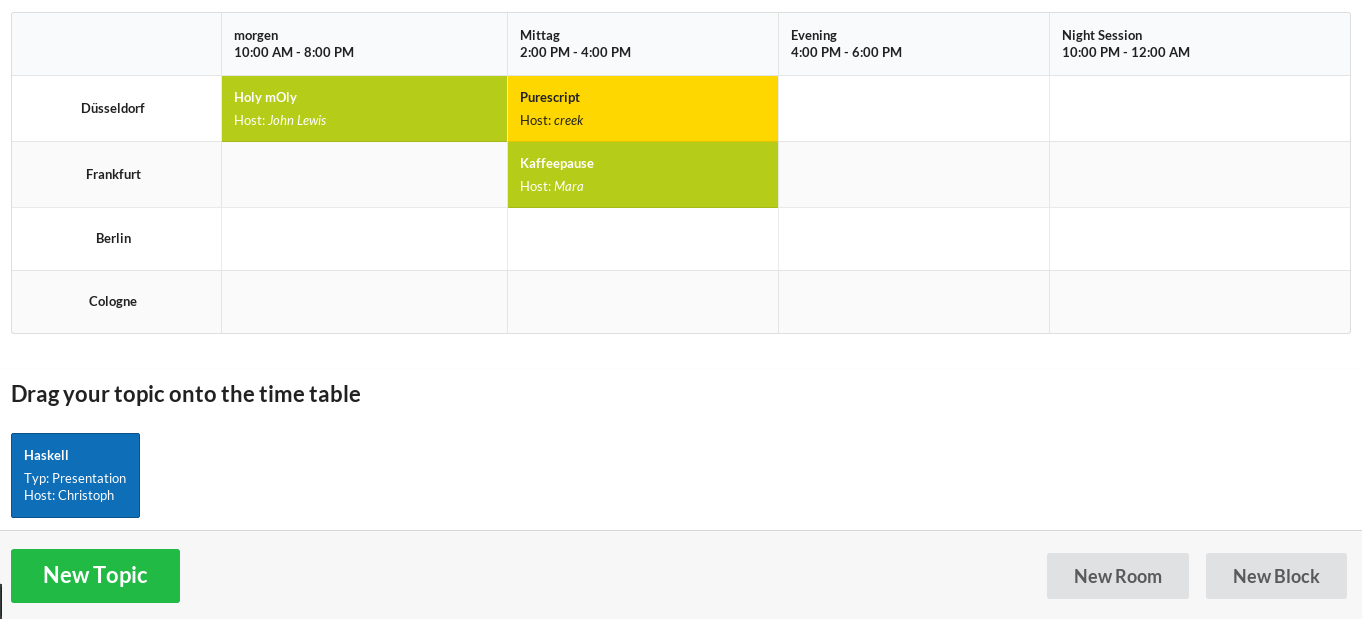
\includegraphics[width=\textwidth]{fig/timetable.png}
  \caption{Zeitplan}
\end{figure}

\subsection{Abschnitte}
Die Zeitplan Ansicht ist in drei visuelle Abschnitte eingeteilt.
\subsubsection*{Das Board}
Das Board ist eine zweidimensionale Matrix, bei der auf der X-Achse die
Zeitslots und auf der Y-Achse die Räume liegen. In den einzelnen Zellen der
Matrix befinden sich Themen die zur Zeit x in Raum y stattfinden.
\subsubsection*{Themenspeicher}
Im Themenspeicher befinden sich Themen die noch keinem Raum und Zeitslots
zugeordnet wurden.
\subsubsection*{Fußzeile}
In der Fußzeile befinden sich Knöpfe zum Anlegen von Räumen, Zeitslots und
Themen.
\subsection{Aktionen}
Auf der Zeitplan Ansicht wird die Planung und Organisation des Open Spaces
durchgeführt. Hierfür werden drei verschiedene Arten von Aktionen unterstützt.
\subsubsection*{Anlegen}
In der Zeitplan Ansicht lassen sich die Räume und Zeitslots der Veranstaltung
anlegen und anpassen. Weiterhin werden in dieser Ansicht neue Themen angelegt
und dem Themenspeicher hinzugefügt. Das Anlegen der Räume, Zeitslots und Themen
wird in Popups mit den nötigen Angaben vorgenommen, die sich durch Klicks auf
die entsprechenden Knöpfe in der Fußzeile aufrufen lassen. Für neue Themen
stehen verschiedene Typen zur Verfügung:
\begin{itemize}
\item Diskussion -- Gelb
\item Präsentation -- Blau
\item Workshop -- Grün
\end{itemize}

\subsubsection*{Verschieben}
Neu angelegte Themen werden zunächst im Themenspeicher abgelegt und können dann
per Drag `n Drop auf das Board gezogen werden. Genauso können Themen auf dem
Board in andere Slots gezogen oder vom Board entfernt werden. Verschiebt man ein
Thema auf ein Feld das bereits belegt war, wird das vorherige Thema in den
Themenspeicher gelegt und das neue Thema dem Feld zugewiesen.

\subsubsection*{Entfernen}
Möchte man ein Thema vollständig löschen, erscheint, sobald man das Thema
angehoben hat, in der Fußzeile eine breiter Löschstreifen der durch ein
Mülltonnen Icon gekennzeichnet ist. Bewegt man ein Thema über diesen Streifen
leuchtet dieser rot auf, und lässt man das Thema dann los, wird es gelöscht.

Weiterhin können auch einmal erstellte Räume und Zeitslots wieder entfernt
werden. Bewegt man die Maus über die entsprechende Felder im Tabellenkopf oder
in der ersten Tabellenspalte, erscheint ein X-Icon bei dessen Klick der
entsprechende Raum oder Zeitslot vom Board entfernt wird.

\section{Administrator Ansicht}
\label{sec:admin-ansicht}
In der Administrator Ansicht werden die verschiedenen
Instanzen verwaltet.
\begin{figure}[ht]
  \centering
  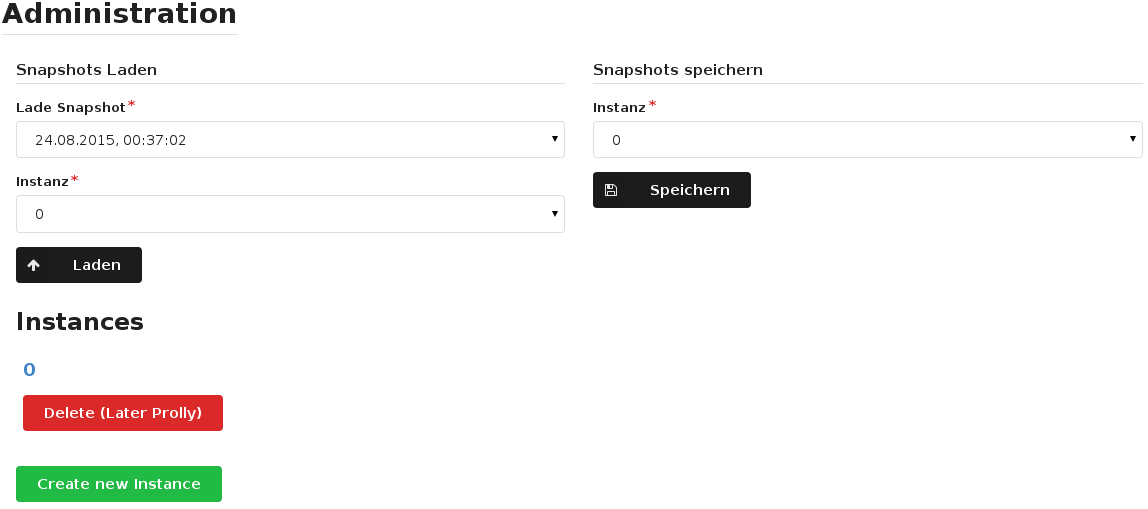
\includegraphics[width=\textwidth]{fig/admin.png}
  \caption{Administration}
\end{figure}

\subsection*{Instanzen}
\label{sec:instanzen}
 Mit einem Klick auf \emph{Create new Instance} kann eine
neue Instanz angelegt werden. Diese wird mit einer UUID verknüpft und kann
anschließend über diese referenziert werden. Mit einem Klick auf eine UUID in
der Instanzliste kann direkt auf das Board dieser Instanz gewechselt werden.

\subsection*{Snapshots}
\label{sec:snapshots}
Unter \emph{Snapshots speichern} kann eine Instanz ausgewählt und ihr
derzeitiger Zustand in einem Snapshot persistiert werden.
Mittels \emph{Snapshots laden} kann dieser sowie früher gespeicherte Snapshots
in eine beliebige Instanz geladen werden. Der Zustand dieser Instanz wird dann
durch den Snapshot ersetzt.

\section{Synchronisierung}

%%% Local Variables:
%%% mode: latex
%%% TeX-master: "../ai-projekt"
%%% End:
